\section{Network properties of Stack Exchange data}

We examine the differences between live and closed communities by analysing network properties and dynamic of collective trust. We are particularly interested in the position of trustworthy members in these communities and whether there are differences between live and close communities. For these reasons, we map the interaction data onto networks and analyse their network properties. We use dynamical reputation model to estimate the trustworthiness of each member of community.     

\subsection{Network mapping}
%{\color{blue} Here we need a description how we map the data onto networks, why sliding windows $30$days, sliding windows, etc....}

%From Stack Exchange data, we selected questions, answers and comments. Each post is associated with the user-id and timestamp. 
%ovo gore sam iskomentarisala zato sto postoji u data sekciji
We treat all user interactions (answering questions, posting questions or comments, accepting answers) as equal. We construct a network of users where the link between two nodes (users) $i$ and $j$ exists if: $i$ answers or comments question posted by $j$ and vice verse, or $i$ comments answer posted by $j$ and vice verse. We do not consider the direction or the frequency of the interaction between users $i$ and $j$, and thus, we create unweighted and uncorrelated network. 
%This is probably not good enough argument…
We study how properties of networks evolve in the first 180 days of the community life. We create a network snapshot $G(t, t+\tau$) at the time $t$ for the time window length $\tau$. Two users $(i, j)$ are connected in a network snapshot $G(t, t+\tau$) if they had at least one interaction during the time $[t,t+\tau]$. We create 150 interaction networks, our first network accounts for interaction within the first 30 days $G[0,30)$ and we slide the window of interaction by one day and finish with $G[149,179)$ network. By sliding the time window by one day we create two consecutive networks that overlap significantly. This way we are able to to capture fine structural changes that are consequences of daily added/removed interactions. We calculate different structural properties of these networks and analyse how they change over the period of 180 days.  


\subsection{Clustering}
There are many local and global measures of network properties \cite{boccaletti2006complex}. These measures are not independent. However, it was shown that degree distribution, degree-degree correlations and clustering coefficient are sufficient to fully describe most of the complex networks including social networks \cite{orsini2015quantifying}. The clustering coefficient of a node quantifies the average connectivity of between its neighbours and cohesion of its neighbourhood \cite{boccaletti2006complex}. It is a probability that two neighbours of a node are also neighbours, and is calculated using the following formula:
\begin{equation}
c_{i}=\frac{e_{i}}{\frac{1}{2}k_{i}(k_{1}-1)} \ .
\label{eq:clust}
\end{equation}
Here $e_{i}$ is the number of links between neighbours of the node $i$ in a network, while $\frac{1}{2}k_{i}(k_{i}-1)$ is the maximal possible number of links determined by the node degree $k_{i}$. The clustering coefficient of network $C$ is the value of clustering averaged over all nodes. Here we investigate how clustering coefficient in a SE community is changing with time by calculating its value for all network snapshots. We compare the behavior of clustering for active and closed communities on the same topic in order to better understand how cohesion of these communities is changing over time. 
Members' clustering coefficient measures the probability that other members connected to them are also connected. Study on dynamics of social group growth shows that that links between one's friends that are members of a social group increase the probability that that individual will join the social group \cite{backstrom2006group}. Furthermore, successful social diffusion  typically occur in networks with high value of clustering coefficient \cite{centola2007cascade}. These results suggest that high local cohesion should be a characteristic of sustainable communities.

We first analyse structural properties of Stack Exchange communities and examine the difference between successful and unsuccessful ones. We calculate the mean clustering coefficient for 30-days window networks and examine how it changes with time. Figure \ref{fig:clustering} shows the evolution of mean clustering coefficient for all eight communities. All communities that are still alive are clustered, with the value of mean clustering coefficient higher than 0.1. Physics, the only launched community, has the value of clustering coefficient above 0.2 for the first 180 days.
During larger part of the observed period, the clustering coefficient of an active community is higher compared to the clustering coefficient of its closed pair. If we compare active communities with their closed counterpart, the closed communities have higher value of the mean clustering coefficient in the early phase while later communities that are still active have higher values of clustering coefficient. These results suggest that all communities have relatively high local cohesiveness, and that lower values of clustering coefficient in the later phase of community life may be an indicator of its decline. 

\begin{figure}
	\centering
	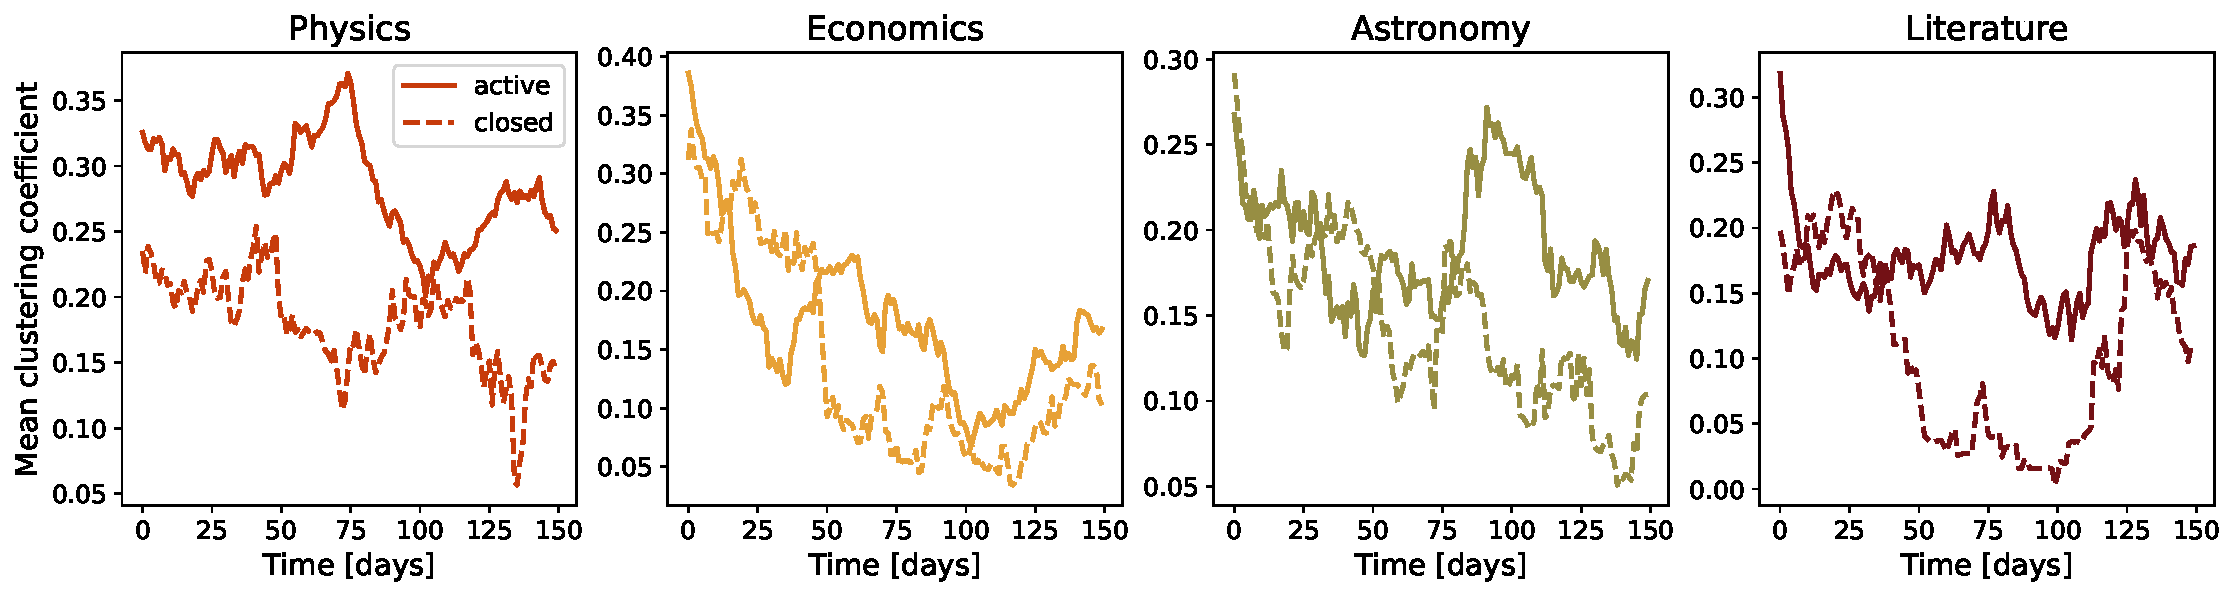
\includegraphics[width=\linewidth]{figures/stackexchange/clustering.pdf}%Figures/figures_SE/Fig3.pdf}
	\caption{Mean clustering coefficient.}
	\label{fig:clustering}
\end{figure}
